\documentclass[12pt, A4]{article}
% font settings
\usepackage[default]{opensans}
\usepackage[onehalfspacing]{setspace}
\usepackage[naustrian]{babel} 
\usepackage[T1]{fontenc}
\usepackage[utf8]{inputenc}
% additional packages
\usepackage{hyperref}
\usepackage{multicol}
\usepackage{graphicx}

\title{ Smart Mirror}
\date{28. April 2020}
\begin{document}
\maketitle

\section{Team}
\begin{center}
\begin{multicols}{2}
\begin{itemize}
	\item[]Patricia Pichler \\ 11850893 
	\item[]Lukas Wais \\ 11816105
	\item[]Jakob Zethofer \\ 01612980
	\item[]Omar Luis Due\~nas Hidalgo \\ 51849509
\end{itemize}
\end{multicols}	
\end{center}

\begin{figure}[h]
\centering
	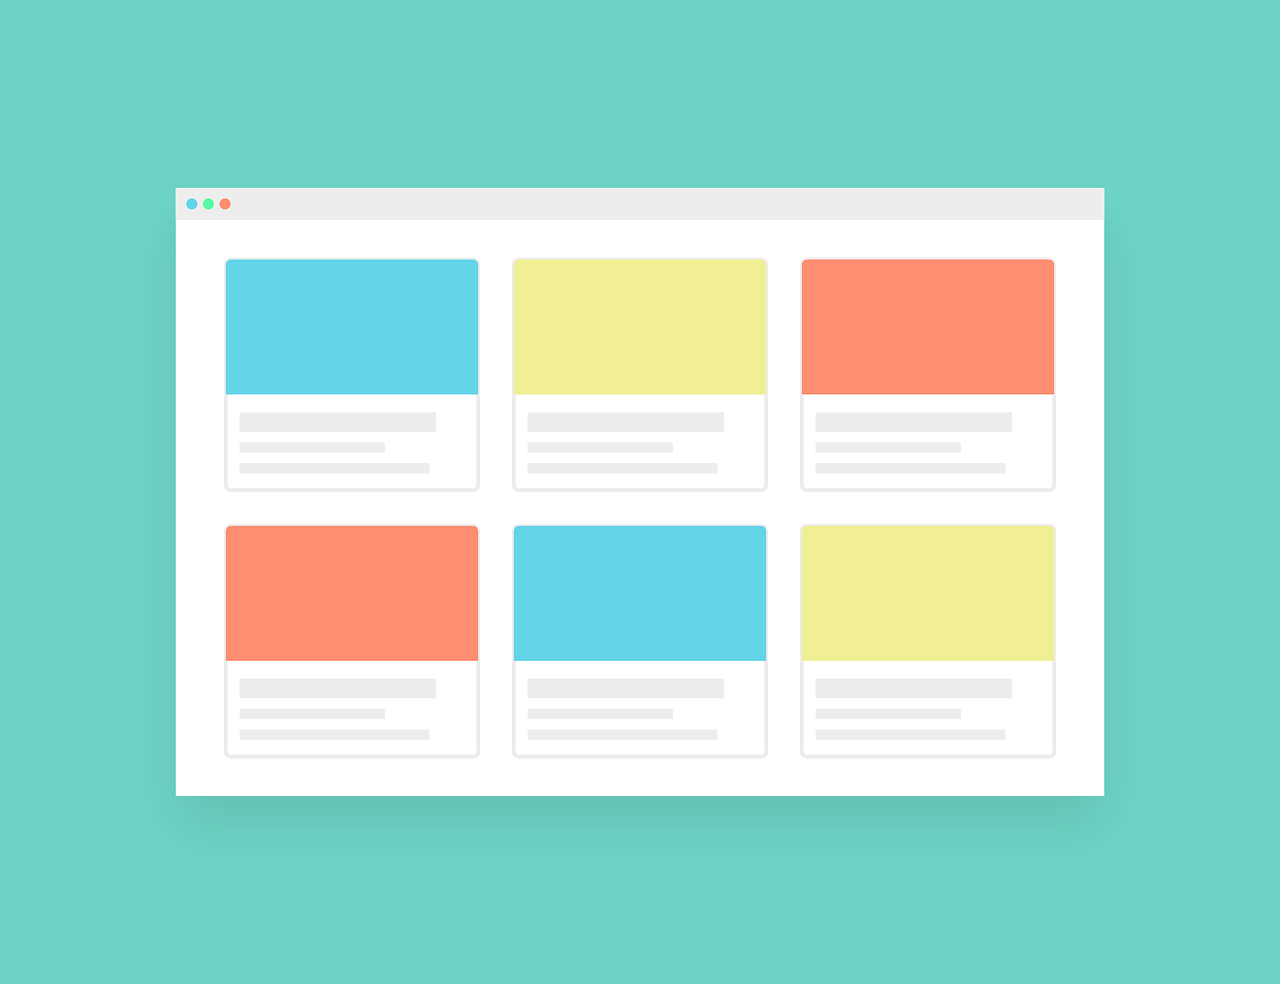
\includegraphics[width=0.6\textwidth]{gui.png}
	\caption{Beispiel GUI \cite{pixabay}}
\end{figure}

\newpage

\section{Features}
\begin{itemize}
	\item Gesichtserkennung
	\item Profile speichern
	\item Kalender anzeigen (Google Konto)
	\item Wetter anzeigen (Standort)
	\item Aktienkurse
	\item Fahrplananzeige
	\item Begrüßung
	\item Animierter Hintergrund
	\item Spracherkennung
\end{itemize}


\section{Projektbeschreibung}
Wir wollen einen Smart Mirror machen, der erkennt, ob eine Person davor steht und dann je nach Person verschiedene Features anzeigt. Pro Person kann ein Profil angelegt werden, in dem die angezeigten Features eingestellt sind. Es kann zum Beispiel der Kalender angezeigt werden, die Aktienkurse einer Börse oder die Abfahrten am nächsten Bahnhof. Dies wird über ein verknüpftes Google-Konto realisiert. Außerdem kann ein Standort über Spracherkennung eingestellt werden, von dem dann das aktuelle Wetter angezeigt wird. Je nach Vorlieben bekommt der Benutzer eine individuelle Begrüßung und kann einen animierten Hintergrund einstellen.

\section{Zielformulierung}
Wir werden versuchen, die oben genannten Ziele mit den unten genannten Technologien umzusetzen. Die niedrigste Priorität wird dabei auf die Spracheingabe gelegt. Wenn sich die Unterscheidung von Gesichtern als zu schwierig herausstellt, werden wir nur unterscheiden, ob jemand da ist und den Profilwechsel manuell umsetzen. 

\section{Realisierung}
\begin{itemize}
	\item Programmiersprache: Java
	\item Oberfläche: JavaFX
	\item Datenbank: Derby DB für Profile
	\item Gesichtserkennung: OpenCV
	\item Spracherkennung: Java Speech API
	\item JavaFX Webview mit HTML Plugins für Wetter, Aktien, Fahrplan, Kalender, \ldots
	\item Animierter Hintergrund: GIF
	\item Sourcecodeverwaltung: Github
\end{itemize}
Über OpenCV soll erkannt werden, ob gerade ein Benutzer vor dem smart mirror steht und nach Möglichkeit auch welcher. Wenn dies der Fall ist werden die dem Benutzer zugeordneten Plugins auf dem Bildschirm angezeigt. Dafür werden wir vor allem Webviews verwenden, die HTML Plugins darstellen. Der Hintergrund wird nur angezeigt, wenn ein Benutzer da ist und ist individuell einstellbar. Die Einstellungen des Benutzers werden in der Datenbank gespeichert. 

 \bibliographystyle{ieeetr}
  \bibliography{cite.bib}
\end{document}







 